\documentclass{endm}
\usepackage{endmmacro}
\usepackage{graphicx}

% The following is enclosed to allow easy detection of differences in
% ascii coding.
% Upper-case    A B C D E F G H I J K L M N O P Q R S T U V W X Y Z
% Lower-case    a b c d e f g h i j k l m n o p q r s t u v w x y z
% Digits        0 1 2 3 4 5 6 7 8 9
% Exclamation   !           Double quote "          Hash (number) #
% Dollar        $           Percent      %          Ampersand     &
% Acute accent  '           Left paren   (          Right paren   )
% Asterisk      *           Plus         +          Comma         ,
% Minus         -           Point        .          Solidus       /
% Colon         :           Semicolon    ;          Less than     <
% Equals        =           Greater than >          Question mark ?
% At            @           Left bracket [          Backslash     \
% Right bracket ]           Circumflex   ^          Underscore    _
% Grave accent  `           Left brace   {          Vertical bar  |
% Right brace   }           Tilde        ~

\newcommand{\Nat}{{\mathbb N}}
\newcommand{\Real}{{\mathbb R}}
\def\lastname{Please list your Lastname here}

\begin{document}

% DO NOT REMOVE: Creates space for Elsevier logo, ScienceDirect logo
% and ENDM logo
\begin{verbatim}\end{verbatim}\vspace{2.5cm}

\begin{frontmatter}

\title{Hoy te convert\'is en (Junior) Data Scientist}

%\author{My Name\thanksref{ALL}\thanksref{myemail}}
\author{Ricardo Colombo}
\author{Diego Santos}
\author{Erik Machicado}
%\address{My Department\\ My University\\ My City, My Country}
\address{Departamento de Computaci\'on\\ Universidad de Buenos Aires\\ C.A.B.A, Argentina}

% \author{My Co-author\thanksref{coemail}}
% \address{My Co-author's Department\\ My Co-author's University\\
%    My Co-author's City, My Co-author's Country} \thanks[ALL]{Thanks
%    to everyone who should be thanked} \thanks[myemail]{Email:
%    \href{mailto:myuserid@mydept.myinst.myedu} {\texttt{\normalshape
%    myuserid@mydept.myinst.myedu}}} \thanks[coemail]{Email:
%    \href{mailto:couserid@codept.coinst.coedu} {\texttt{\normalshape
%    couserid@codept.coinst.coedu}}}

% \begin{abstract}
% This is a short example to show the basics of using the ENDM style
% macro files. Ample examples of how files should look may be found
% among the published volumes of the series at the ENDM home page
% ({\texttt{http://www.elsevier.com/locate/endm}})
% \end{abstract}

\begin{abstract}
El trabajo consiste en aplicar t\'ecnicas de M\'etodos num\'ericos y 
Data Science, en particular Regresiones Lineales y Cuadrados M\'inimos, 
a un gran conjunto de datos reales, buscando identificar modelos 
capaces de predecir comportamientos .
\end{abstract}

\begin{keyword}
Data Science, KPIs, Cuadrados Minimos Lineales (CML)
\end{keyword}

\end{frontmatter}


\section{Introducci\'on}\label{intro}

%Contendrá una breve explicación de la base teórica que fundamenta los métodos involucrados en el trabajo, junto con los métodos mismos. No deben incluirse demostraciones de propiedades ni teoremas, ejemplos innecesarios, ni definiciones elementales (como por ejemplo la de matriz simétrica). En vez de definiciones básicas es conveniente citar ejemplos de bibliografía adecuada. Una cita vale más que mil palabras

En la competitiva industria aeron\'autica la eficiencia de los procesos es vital para mantener la calidad del servicio. Cumplir con el servicio no es algo que solo dependa de la empresa que se contrata, ya que año a año la cantidad de vuelos se multipilica y muchas veces existen variables externas que terminen afectando la puntualidad y calidad del servicio. Por eso es importante contar con m\'etricas que analizen los eventos pasados buscando patrones e intentar prevenirlos o desminuir su impacto en el futuro. Estos indicadores son denominados \textit{Key Performance Indicators} (KPIs).

En este trabajo estudiaremos factores que influyen en la organización de las salidas de vuelos para un aeropuerto en particular. Como se mencion\'o anteriormente estad\'isticamente, todos los años se registran mas vuelos para cualquier aeropuerto, esto requiere una sincronizaci\'on precisa de los tiempos que ocupa un avi\'on dentro del aeropuerto esperando para partir.

Para la realización del trabajo analizaremos un set de datos reales correspondientes a vuelos realizados en Estados Unidos durante el per\'iodo 1987 - 2008. Y para poder relacionar los casos utilizaremos en los dos ejes el mismo aeropuerto.

Nuestro primer eje de estudio es la evoluci\'on en la cantidad de tr\'afico \'aereo de un aeropuerto, y como la cuota de \textit{market share} se fue concentrando con el correr del tiempo sobre las empresas l\'ideres del segmento. Lo interesante de esta evaluaci\'on es esperamos poder proyectar el crecimiento de tr\'afico sobre el aeropuerto a fin de poder satisfacer la creciente demanda.

El segundo eje de estudio se centra en los factores estacionales que influyen en un vuelo salga en tiempo y forma, es decir estudiaremos la cantidad de retrasos en partidas para un aeropuerto particular, con el objetivo de detectar las estaciones anuales donde el clima pueda afectar el funcionamiento del aeropuerto.

Luego relacionaremos los ejes de estudio para estudiar si es posible predecir temporadas de mayor retraso, esperando que sea de utilidad en la programaci\'on de los nuevos vuelos que se incorporán al mercado.


%breve explicacion de metodo
\paragraph{Metodo de Minimos Cuadrados}

Minimos cuadrados es una t\'enica de an\'a num\'erico, en la que, dados un conjunto de pares intenta encontrar la funci\'on que mejor aproxime a los datos de acuerdo con el criterio de Error cuadr\'atico medio. En su forma m\'as simple, intenta minimizar la suma de los cuadrados de las diferencias entre los puntos generados por la funci\'on de aproximaci\'on y los que corresponden a los datos. CML es el caso en el que se usa a las rectas para la aproximaci\'on osea $y = ax + b$, adem\'as la generalizaci\'on del m\'etodo propone encontrar la funci\'on que mejor aproxima de la forma $y = a_1f_1(x) + \dots + a_Kf_K(x)$ y que no es necesario que las funciones $f$ sean lineales pero si que $y$ sea una combinaci\'on lineal de ellas. Para mas informacion consultar  \cite{bf} (seccion 8.1)

\section{Desarrollo}
	%Deben explicarse los métodos numéricos que utilizaron y su aplicación al problema concreto involucrado en el trabajo práctico. Se deben mencionar los pasos que siguieron para implementar los algoritmos, las dificultades que fueron encontrando y la descripción de cómo las fueron resolviendo. Explicar también cómo fueron planteadas y realizadas las mediciones experimentales. Los ensayos fallidos, hipótesis y conjeturas equivocadas, experimentos y métodos malogrados deben figurar en esta sección, con una breve explicación de los motivos de estas fallas (en caso de ser conocidas).

	Como se dijo previamente, comenzamos con un set de datos relacionados a los vuelos realizados en Estados Unidos entre 1987 y 2008 (descripto en \cite{d}), luego seleccionamos aquellos datos relacionados con el aeropuerto JFK, entonces propucimos como aspectos a analizar, ver el numero de vuelos con Weather Delay mayor a 15min por mes y la cantidad de vuelos por mes de un conjunto aerolineas de similares caracteristicas (Delta, American y United). Posteriormente con los datos de esos ejes de estudio ya obtenidos para un periodo de tiempo vamos a aplicar el metodo propuesto por la catedra, dicho metodo encontrara la combinacion lineal de funciones (propuestas por el grupo) que mejor aproxime a los datos, con esta combinacion de funciones veremos si tambien aproxima a los resultados de los ejes de estudio para un periodo de tiempo posterior

	Para evitar caer en el conocido overfitting elegiremos distintos subconjuntos del trainig del training para hallar los coeficientes de la aproximacion lineal.


	Al momento de analizar que funciones utilizar en el metodo, como primer opcion se propuso a los polinomios, pues estos fueron estudiados y usados en clase en la introduccion del metodo. Posteriormente se plateo el uso de senos y cosenos, ya que al ser funciones periodicas podrian presentar alguna ventaja si los datos presentan patrones que se repiten varias veces.

\section{Resultados}

	\begin{center}
	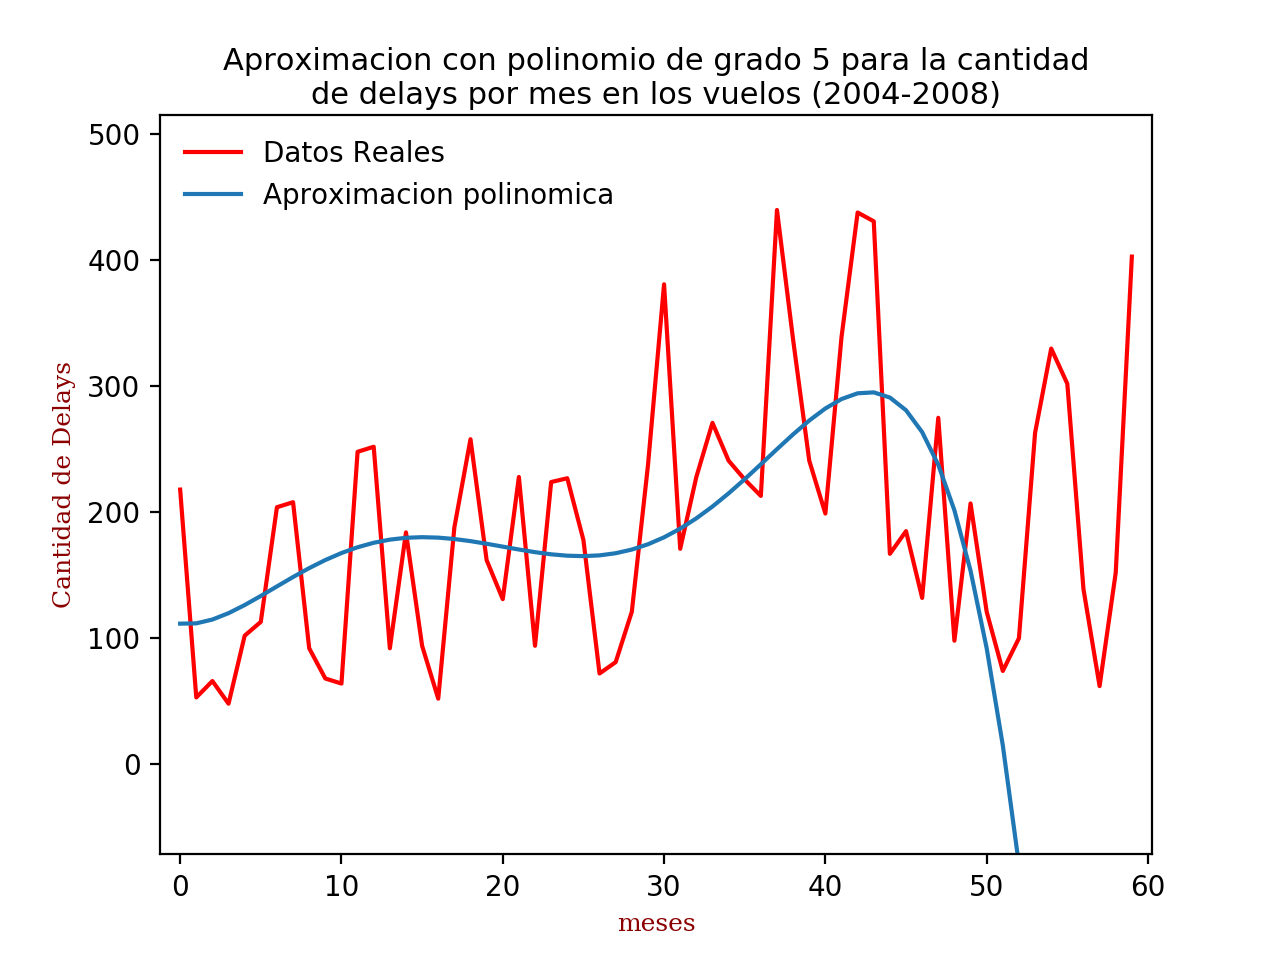
\includegraphics[scale=0.8]{imagenes/delaysPolinomio.png}
	\end{center}
	%porque parece la aproximacion tan lineal?

	

	\begin{center}
	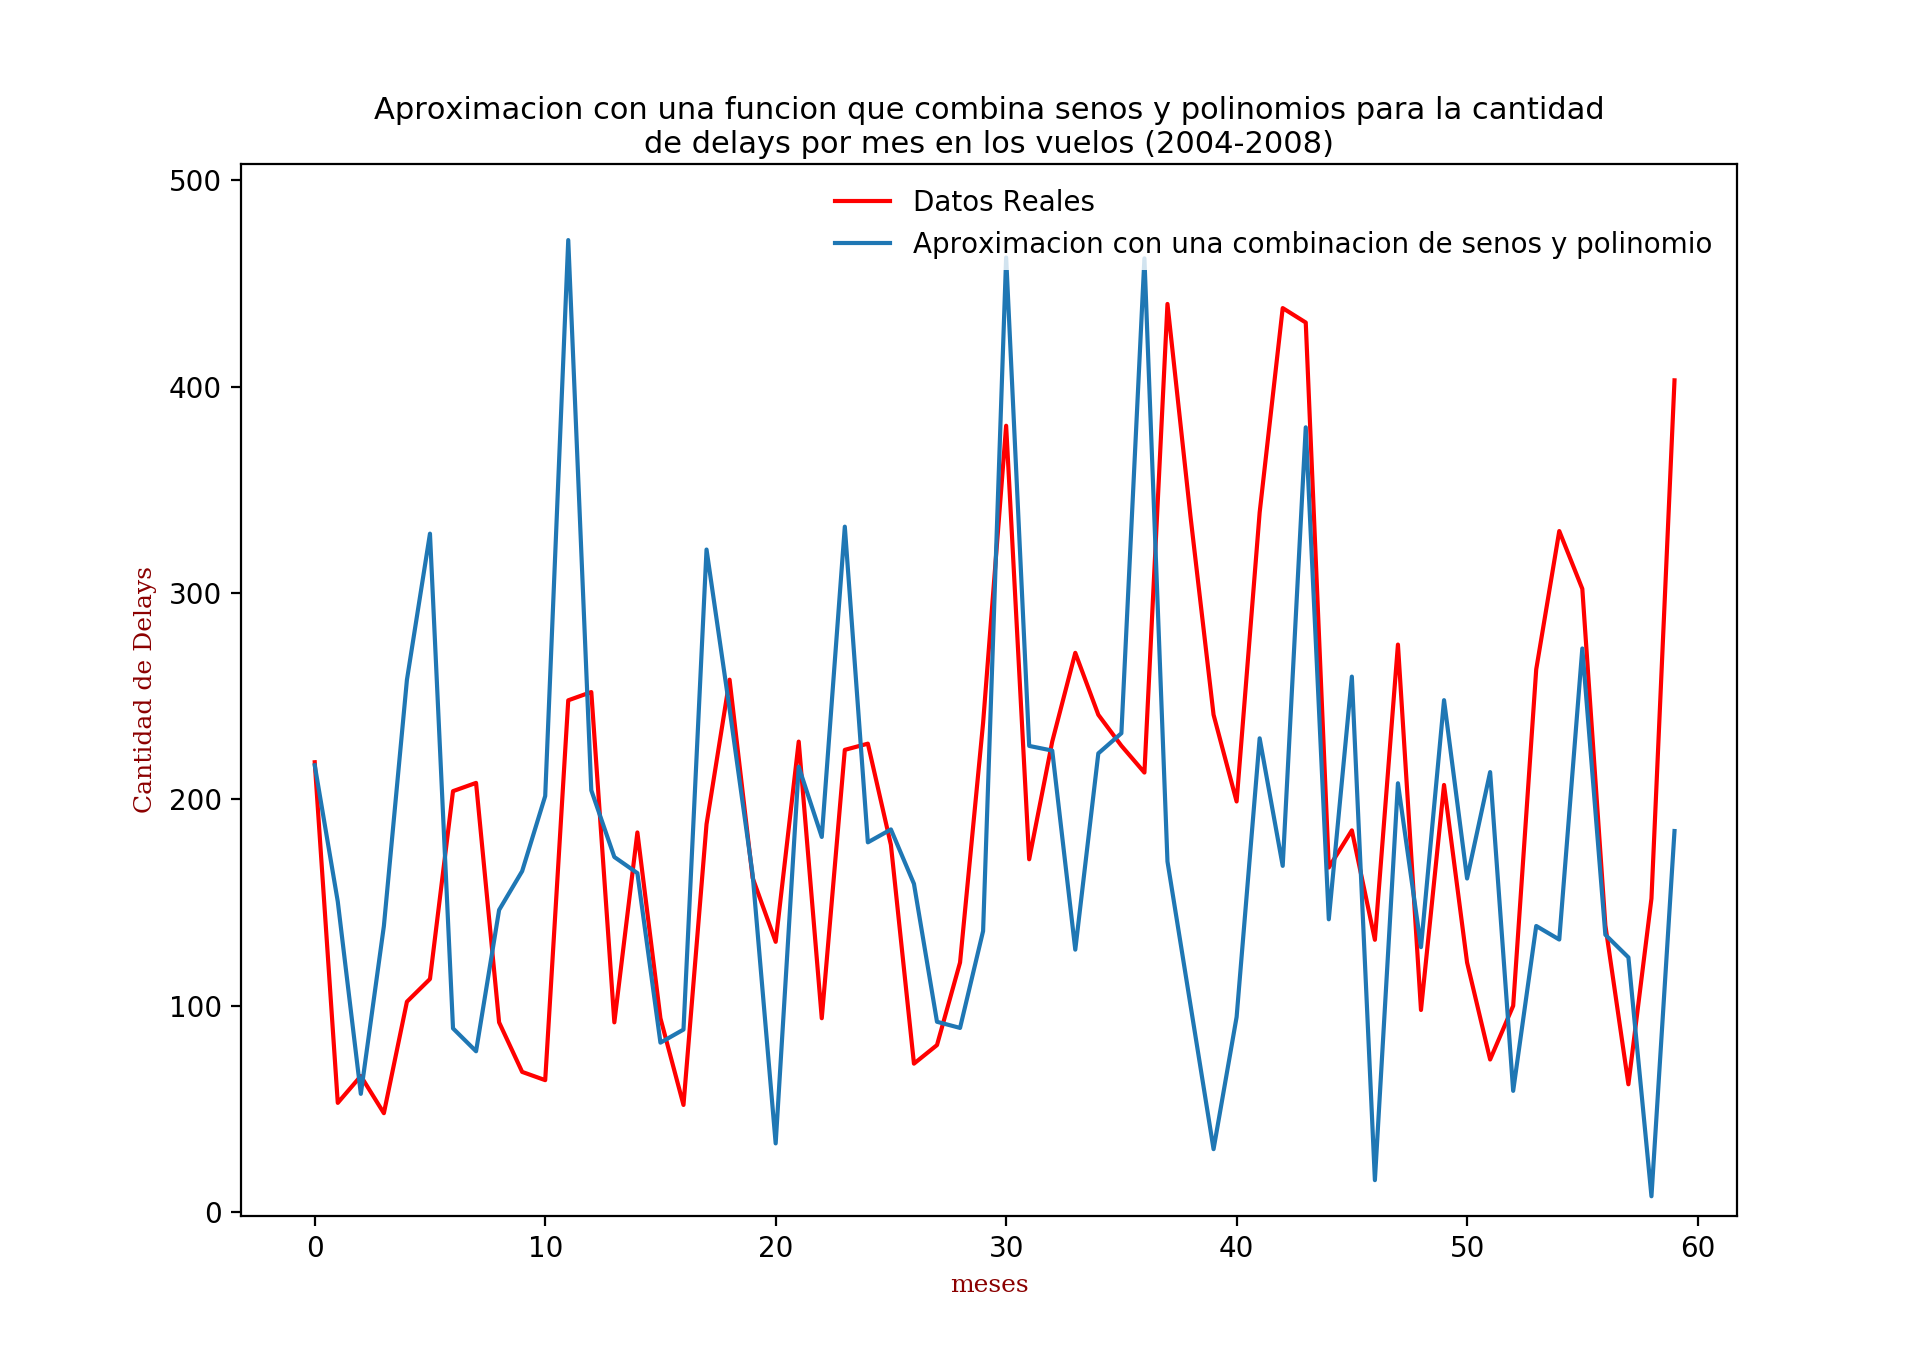
\includegraphics[scale=0.5]{imagenes/polinomioysenos.png}
	\end{center}

	\begin{center}
	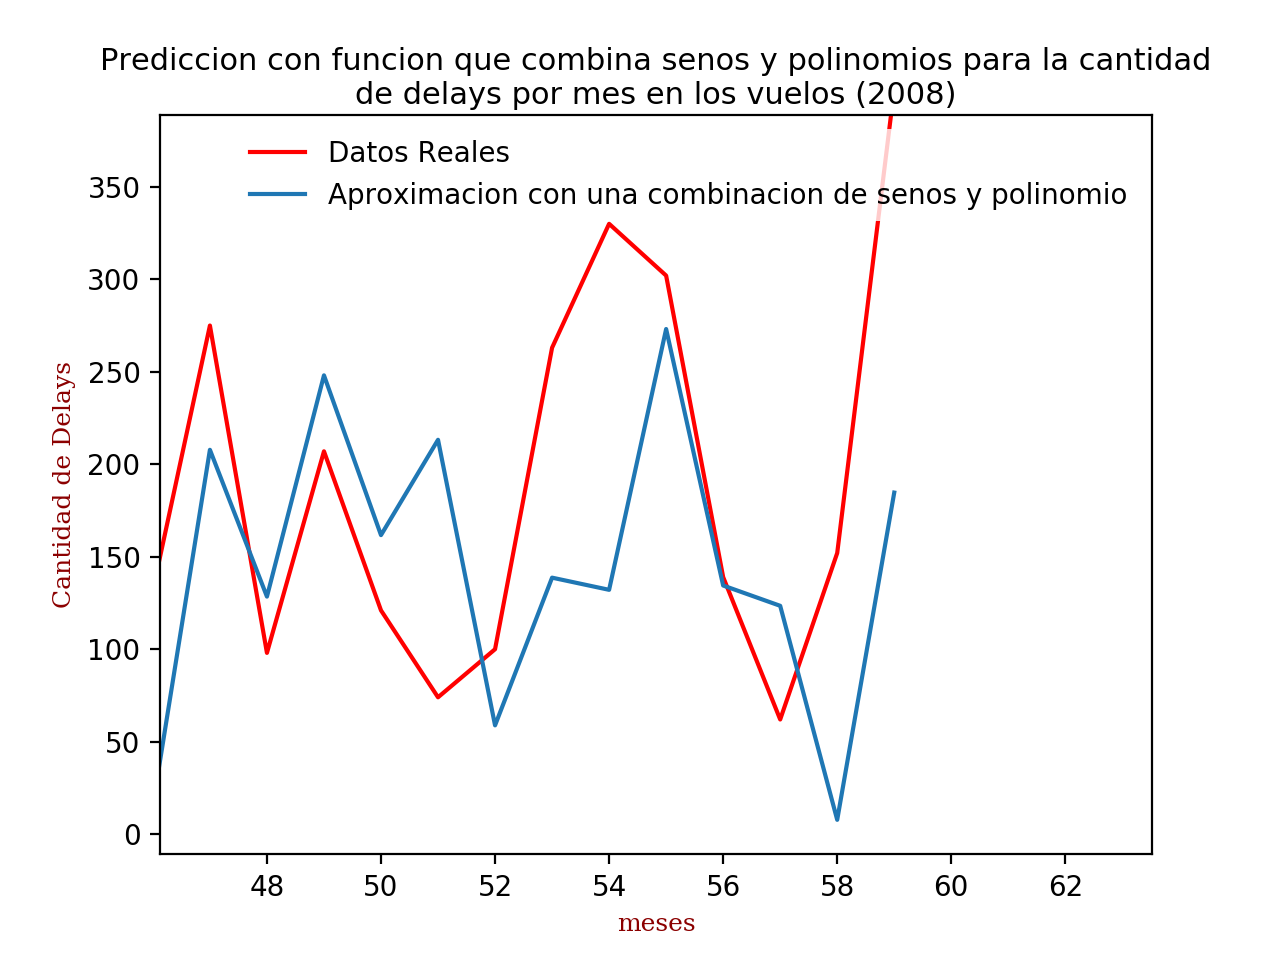
\includegraphics[scale=0.8]{imagenes/delays2008.png}
	\end{center}

\section{Discusi\'on}
	%Hablar de las limintaciones de cada tipo de funcion 
	Durante la experimentacion con la familias de polinomios usadas para el metodo se encontro que si bien en los meses tomados como training se comportaban bastante bien afuera de ese periodo crecia constantemente. 
	%como se muestr acontinuacion

\section{Conclusiones}
	%Hablar sobre la funcion final que escogimos y como reune los que queremos de la dos funciones



\section{Summary and Remarks}

The ENDM macro package is relatively easy to use and provides a
uniform layout for all the papers that appear in ENDM.

\paragraph{Assigning Volume Numbers}

An additional point worth mentioning is that ENDM has moved to
\emph{ScienceDirect}, Elsevier's main platform for publishing
electronic series. Because \emph{ScienceDirect} cannot easily
accommodate changes to published material, the \emph{Proceedings}
must be entirely ready before they can be published. Volume numbers
will therefore not be assigned for the \emph{Proceedings} until the
final versions of all papers are in.

\paragraph{Copyright Transfer Forms}

Due to the move to \emph{ScienceDirect}, the corresponding author of
each paper published in ENDM must submit a signed Copyright Transfer
Form to Elsevier in order for their paper to be published. A copy of
this form will be sent to each author. Note that the publication of
an abstract or extended abstract in ENDM will not restrict the
author(s) from publishing a full-length article on the same topic and
with the same title in another journal (possibly with another
publisher). Details about the copyright agreement specifying the exact
rights of the authors and the rights of Elsevier are available at
\href{http://authors.elsevier.com/PublisherInfoDetail.html?dc=AGI}
{Elsevier's Author Gateway}.


\section{Bibliographical references}\label{references}

ENDM employs the \texttt{plain} style of bibliographic references in
which references are numbered sequentially and listed in alphabetical
order according to the first author's last name. Please utilize this
style. We have a Bib\TeX\ style file, for those who wish to use it.
It is the file \texttt{endm.bst} which is included in this package.
The basic rules we have employed are the following:
\begin{itemize}
\item Authors' names should be listed in alphabetical order, with the
first author's last name listed first followed by initials or first
name, and with the other authors' names listed as \emph{first name,
last name}.
\item Titles of articles in journals should be in \emph{emphasized}
font.
\item Titles of books, monographs, etc.\ should be in quotations.
\item Journal names should be in plain roman type.
\item Journal volume numbers should be in boldface, immediately
followed by the year of publication enclosed in parentheses in
roman type.
\item References to URLs on the net should be ``active'' and the URL
itself should be in {\tt typewriter} font.
\item Articles should include page numbers.
\end{itemize}

The criteria are illustrated by the examples below.


\begin{thebibliography}{10}\label{bibliography}

\bibitem{cy} Civin, P., and B. Yood, \emph{Involutions on Banach
    algebras}, Pacific J. Math. \textbf{9} (1959), 415--436.
  
\bibitem{bf} Burden, R. L., and J. D. Faires, ``An\'alisis num\'erico,
'' Math. Surveys \textbf{7}, Amer. Math. Soc.,
  Providence, R.I., 1961.
  
\bibitem{d} ASA Section on Statistical Computing. 2009 data expor competition, URL:
  \href{http://stat-computing.org/dataexpo/2009/the-data.html}
  {\texttt{http://stat-computing.org/dataexpo/2009/the-data.html}}.
  
\bibitem{em2} Easdown, D., and W. D. Munn, \emph{Trace functions on
    inverse semigroup algebras}, U. of Glasgow, Dept. of Math.,
  preprint 93/52.

\bibitem{r} Roscoe, A. W., ``The Theory and Practice of Concurrency,''
  Prentice Hall Series in Computer Science, Prentice Hall Publishers,
  London, New York (1198), 565pp. With associated web site\\  
  \href{http://www.comlab.ox.ac.uk/oucl/publications/books/concurrency/}
  {\texttt{http://www.comlab.ox.ac.uk/oucl/publications/books/concurrency/}}.
  
\bibitem{s} Shehadah, A. A., ``Embedding theorems for semigroups with
  involution, `` Ph.D.  thesis, Purdue University, Indiana, 1982.
  
\bibitem{w} Weyl, H., ``The Classical Groups,'' 2nd Ed., Princeton U.
  Press, Princeton, N.J., 1946.

\end{thebibliography}

\end{document}
